\documentclass{exam}
\usepackage[utf8]{inputenc}
\usepackage{amsmath,amsthm,geometry,amssymb,enumerate}
\usepackage{graphicx}

 
\begin{document}
 
\begin{center}
\fbox{\fbox{\parbox{5.5in}{\centering
Math 1314  \hfill Final Exam (Choose any 10)\hfill May 2018 \\Answer the questions in the spaces provided.}}}
\end{center}
 
\vspace{5mm}
 
\makebox[\textwidth]{Name and Time:\enspace\hrulefill}
 
\vspace{5mm}
 
\makebox[\textwidth]{G-Number:\enspace\hrulefill}
 
\begin{questions}
	
	\question 
	\subitem a) Solve \quad \quad \quad  \hfill\enspace\hrulefill $$\frac{5}{2x-3}=\frac{3}{x+5}$$
	\vspace{5cm}
	
	\subitem b) Solve the inequality \quad \quad \quad  \hfill\enspace\hrulefill $$|3t-2|\leq 4$$
	\vspace{5cm}
	
	\subitem c) Solve \quad \quad \quad  \hfill\enspace\hrulefill $$x^2+4x+4=0$$
	\vspace{5cm}
	
	\question Find the x- intercept, y - intercept, check for symmetry, also plot the graph for   $y = x^2-2$
	\hfill\enspace\hrulefill
	\clearpage
	
	\question 
	\subitem a) Check whether following two lines are parallel, perpendicular or neither? \\ \(y=2x-3 \quad \mbox{and} \quad y=2x+4\) \hfill\enspace\hrulefill 
	\vspace{4cm}
	
	\subitem b) Find the Equation of the circle with center  \((h,k)=(-5,-2)\) and radius \(r=7\).
	\hfill\enspace\hrulefill 
	\vspace{6cm}
	
	\subitem c) For \(f(x)=3x+4, g(x)=2x-3\) find the following
	\subitem i) Find f(0),\quad  ii) g(1), 
	\hfill\enspace\hrulefill 
	\vspace{7cm}
	
	\question 
	\subitem a) Write down the augmented matrix for the system of equations
	\begin{align}
	\nonumber
	2x+y-3z=&0 \\ 
	\nonumber
   -2x+2y+z=&-7 \\ 
   \nonumber
	3x-4y-3z=&7  
	\end{align}
	 \vspace{6cm}
	

	
	 
	\subitem b) Solve the system of equation by matrix method
	\hfill\enspace\hrulefill
	\begin{align}
	\nonumber
	x+y=&8 \\ 
	\nonumber
	x-y=&4   
	\end{align}
	\vspace{6cm} 
	
		
	
	\clearpage
	\question 
	\subitem a) Is $f(x) =\frac{2}{5+x}$ is one to one? Give reason. 
	\hfill\enspace\hrulefill 
	\vspace{7cm}
	
	
	\subitem b) Find the inverse of the following one-one function, $f(x)=2x+3 $
	\hfill\enspace\hrulefill 
	\vspace{\stretch{1}}
	
	
	
	\clearpage
					
	\question  
	\subitem a) Solve for the x,\quad \(3^{x}=81\) \hfill\enspace\hrulefill 
	\vspace{6cm}
	
	
	\subitem b) Solve for the x,\quad \( 4^{2x+3}=\frac{1}{4}\) \hfill\enspace\hrulefill 
	\vspace{6cm}
	
	\subitem c) Solve for the x,\quad \(log_3(x)=2\) \hfill\enspace\hrulefill 
	\vspace{6cm}
	
	\subitem d) Solve for the x,\quad \( log_6(36)=5x+3\) \hfill\enspace\hrulefill 
	\vspace{6cm}
		
	
	\question  
	\subitem a) Find the exact value of \subitem i) \(log_8(8)\)\\
	 \vspace{3cm}
   \subitem	ii) \(log_3(27)\)
	\vspace{3cm}
	\subitem b)  If $f(x) =\frac{2}{3+x} \mbox{and} g(x)=3x$ then find  
	\hfill\enspace\hrulefill
	\subitem a) $f\circ g(x)$. 
	\vspace{3cm}
	\subitem a) $f\circ g(0)$. 
	\vspace{3cm}
	
		
	
	\clearpage
	\question Use the properties of logarithm to express as sum and difference 
		
	\subitem a) \(log_{2}(4x^3)\) \hfill\enspace\hrulefill 
	\vspace{\stretch{0.1}}
	
	\subitem d) \(ln(4xe^x)\) \hfill\enspace\hrulefill 
	\vspace{\stretch{0.1}}

	\question  
	\subitem a)Two friends decide to meet in Houston for the Texans game next weekend.  Deanna travels 231 miles in the same time that John travels 213 miles. Deanna's trip uses more interstate highways and she can average 6 mph more than John. What is Deanna's average speed?
	\hfill\enspace\hrulefill 
	\vspace{\stretch{0.5}}
	
	\subitem b) The manager of a coffee shop has one type of coffee the sells for $\$5$ per pound and another that sell for $\$14$ per pound. The manager wishes to mix 30 pounds of the $\$14$ coffee to get a mixture that will sell for $\$10$ a pound. How many pounds of the $\$5$ coffee should be used?
	
	
	
	
	
	\clearpage
	\question 
	\subitem a) Find the vertical, horizontal Asymptotes, x-intercept, and Y-intercept (if any) for  
	\hfill\enspace\hrulefill $$f(x)=\frac{x-2}{x^2-4x+4}$$
	\vspace{\stretch{0.1}}
	 
	\subitem b) Find the domain of $y=\frac{2x-3}{x^2-4}$
	\hfill\enspace\hrulefill 
	\vspace{\stretch{0.1}}
	
	\question 
	\subitem a) Find the zeros of f(x) by using rational zeros theorem 
	\hfill\enspace\hrulefill $$f(x)=x^3-2x^2-x+2$$
	 \vspace{7cm}
	 \subitem b) use the following graph to answer the following
	 \begin{figure}[http!]
	 	\centering
	 	\hspace*{0.9cm} 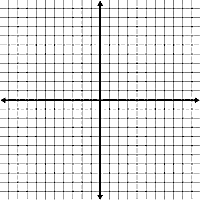
\includegraphics[height=9.0cm,width=12.5cm,angle=0]{graph1.png}
	 	\caption{Graph}
	 \end{figure}
	 
	 
	 \subitem i) find $f(\pi)$
	 \subitem ii) domain of the function
	 \subitem iii) interval where the $f(x) $ is increase and where $f(x) $ is decreasing. 
	 
	 \clearpage
	 \question 
	 \subitem a) Draw the following graph
	 \begin{figure}[http!]
	 	\centering
	 	\hspace*{0.9cm} \includegraphics[height=9.0cm,width=12.5cm,angle=0]{graph2.png}
	 	\caption{Graph}
	 \end{figure}
	 \vspace{5cm}
	 
	
	 \subitem b) For \(g(x)=x^2\) Sketch the graph  and Write down the function for each problems from a) to d) 
	 \subitem a) 3 unit shifting up
	 \subitem b) 2 unit shifting left
	 \subitem c) 1 unit shifting right
	 \subitem d) 4 unit shifting down
	 
	
	\question 	\subitem a) Solve the system by using inverse matrix method .\hfill\enspace\hrulefill
	\begin{align}
	\nonumber
	x+3y=&5 \\ 
	\nonumber
	2x-3y=&-8   
	\end{align}
	Note that 
		\begin{align}
		\nonumber
		\begin{bmatrix}
		1 &   3&  \\
		2 &   -3&  
		\end{bmatrix}^{-1}=
		\begin{bmatrix}
		\frac{1}{3} &   \frac{1}{3}&  \\
		\frac{2}{9} &   -\frac{1}{9}&  
		\end{bmatrix}
		\end{align}
		
		\vspace{\stretch{1}}
		\clearpage
\end{questions}
\clearpage
\end{document}